\documentclass[11pt,letterpaper]{article}
\PassOptionsToPackage{hyphens}{url}
\usepackage[margin=.83in,top=.8in,bottom=.8in,headheight=15pt]{geometry}
\usepackage[T1]{fontenc}
\usepackage{lmodern,amsmath,amssymb,mathtools,bm,booktabs,array,graphicx,tikz}
\usetikzlibrary{arrows.meta,positioning,calc,decorations.pathreplacing,patterns}
\definecolor{ink}{HTML}{17344D}\definecolor{accent}{HTML}{087E8B}\definecolor{pale}{HTML}{EDF5F5}\definecolor{gold}{HTML}{AD6B19}
\providecommand{\dd}{\,\mathrm{d}}\providecommand{\R}{\mathbb{R}}
\providecommand{\E}{\mathbb{E}}\providecommand{\Var}{\operatorname{Var}}
\providecommand{\Cov}{\operatorname{Cov}}\providecommand{\diag}{\operatorname{diag}}
\providecommand{\norm}[1]{\left\lVert#1\right\rVert}
\providecommand{\abs}[1]{\left|#1\right|}
\usepackage{microtype,hyperref,fancyhdr,enumitem,amsthm,sectsty,needspace}
\allsectionsfont{\raggedright}
\hypersetup{colorlinks=true,linkcolor=ink,urlcolor=accent,pdfauthor={Zan Ahmad},pdftitle={Feedback, stability, and hydrostatic pressure / Lecture notes}}
\setlength{\parindent}{0pt}\setlength{\parskip}{6pt}\linespread{1.07}
\setlist{itemsep=3pt,topsep=4pt,leftmargin=*}
\emergencystretch=2em\clubpenalty=10000\widowpenalty=10000
\pagestyle{fancy}\fancyhf{}\fancyhead[L]{\small Mathematical Cardiology}\fancyhead[R]{\small Lecture 6}
\fancyfoot[L]{\footnotesize Zan Ahmad}\fancyfoot[R]{\footnotesize\thepage}\renewcommand{\headrulewidth}{.3pt}
\newtheorem{proposition}{Proposition}\newtheorem{theorem}{Theorem}\newtheorem{lemma}{Lemma}
\theoremstyle{definition}\newtheorem{definition}{Definition}\newtheorem{example}{Example}
\numberwithin{equation}{section}
\begin{document}
{\small\scshape Mathematical Cardiology\hfill Lecture 6}\par\medskip
{\raggedright\hyphenpenalty=10000\exhyphenpenalty=10000\LARGE\bfseries\color{ink} Feedback, stability, and hydrostatic pressure\par}\medskip
{\small Lecture notes}\par\bigskip
A regulated quantity need not remain fixed when its environment changes. Regulation means that a change is measured and used to alter a mechanism that influences the quantity. We shall make this statement quantitative for a deliberately small pressure controller. The calculation will distinguish three questions: whether the desired pressure is an equilibrium, whether the updates approach that equilibrium, and whether the available range of heart rates makes the equilibrium attainable.

\section{Closing the pressure loop}
\hypertarget{note-closing-the-pressure-loop}{}\label{note:closing-the-pressure-loop}
{\small \href{slides.html\#frame=pressure-as-a-function-of-rate\&step=1}{Slides for this section}}\par
Let $H$ denote heart rate in beats per minute and let $V_s$ denote the volume ejected per beat in milliliters. If every beat ejects the same volume, the mean flow in liters per minute is
\begin{equation}Q=\frac{HV_s}{1000}.\end{equation}
We retain a single passive resistance $R$ between arterial pressure $P$ and a fixed downstream pressure $P_v$. Hence
\begin{equation}P=P_v+RQ=P_v+\frac{RV_s}{1000}H.\label{eq:pressure-rate}\end{equation}
This relation contains no storage or pulsation. It assigns a mean pressure immediately to a chosen rate and resistance. In particular, changing rate here cannot alter stroke volume; that is an assumption, rather than a property of the heart.

Take $V_s=100\,\mathrm{mL/beat}$, $P_v=5\,\mathrm{mmHg}$, $R=15\,\mathrm{mmHg\,min/L}$ and $H=60\,\mathrm{beats/min}$. Then $Q=6\,\mathrm{L/min}$ and $P=95\,\mathrm{mmHg}$. If resistance falls to $10$ while rate remains fixed, the pressure becomes $65\,\mathrm{mmHg}$. The immediate $30\,\mathrm{mmHg}$ error supplies a signal for the controller. It does not yet tell us how quickly, or even whether, that controller will correct the error.
\begin{center}\begin{minipage}{.98\linewidth}\centering
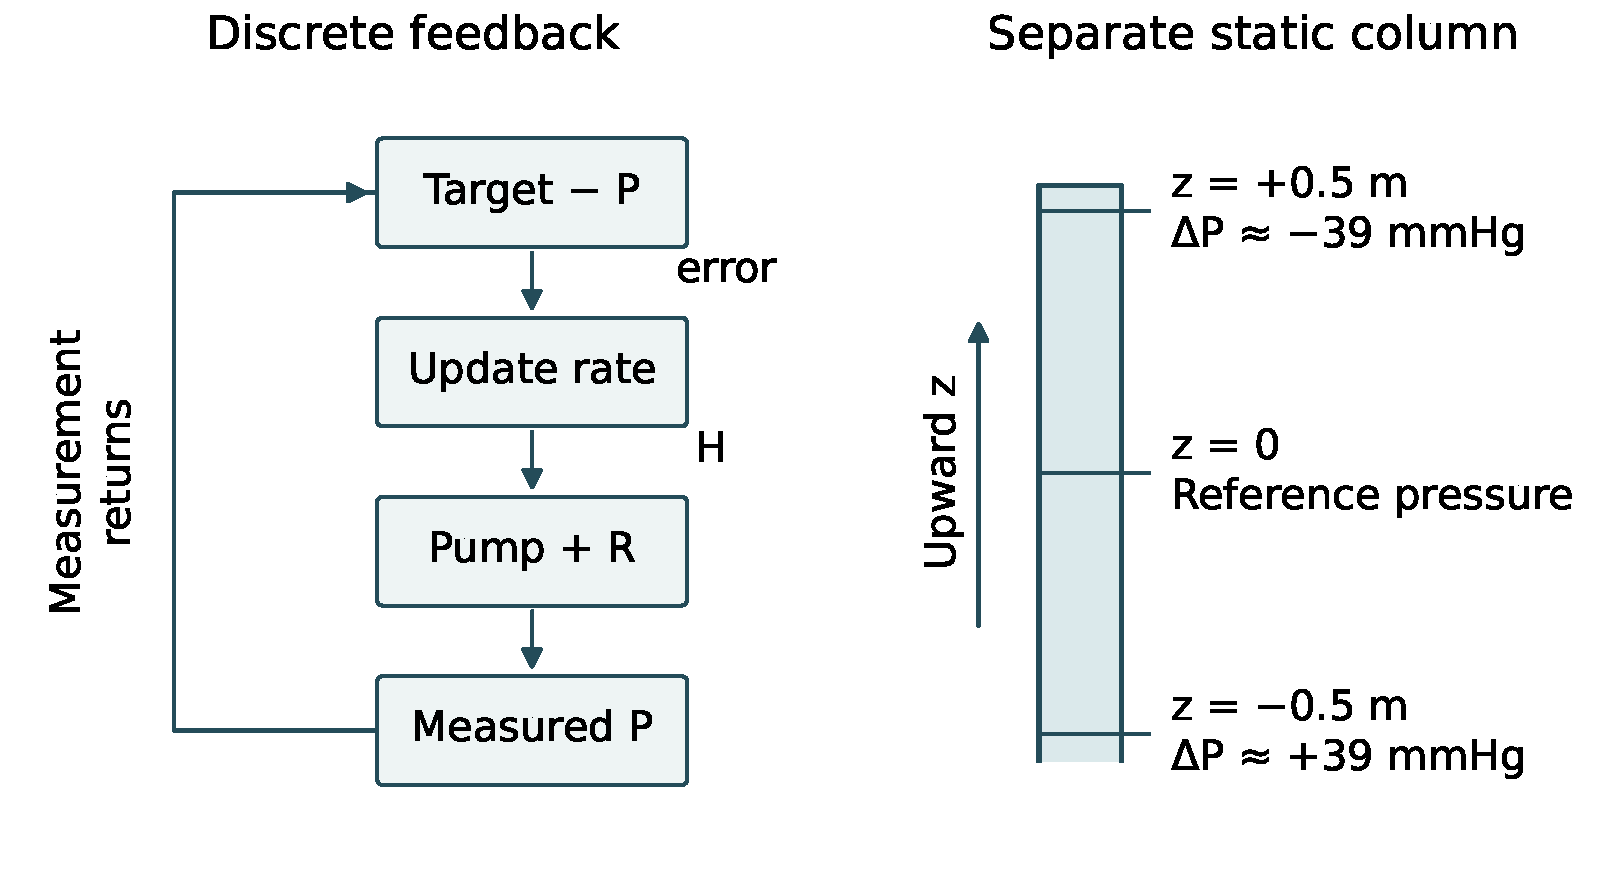
\includegraphics[width=.96\linewidth,height=.57\textheight,keepaspectratio]{feedback-and-height.pdf}\par\smallskip
{\small Original diagrams. The feedback schematic defines a discrete rate controller; the static column uses rho =\allowbreak{} 1060 kg/m$^3$ and g =\allowbreak{} 9.81 m/s$^2$. Height is not an input to the supplied recurrence.}
\end{minipage}\end{center}
\section{A discrete correction rule}
\hypertarget{note-a-discrete-correction-rule}{}\label{note:a-discrete-correction-rule}
{\small \href{slides.html\#frame=a-measured-error-changes-the-next-rate-figure\&step=1}{Slides for this section}}\par
Write $P_*$ for the desired pressure and $H_n$ for the rate at update $n$. Define
\begin{equation}a=\frac{RV_s}{1000},\qquad P_n=P_v+aH_n.\end{equation}
The coefficient $a$ has units of pressure per unit heart rate. The unconstrained correction rule is
\begin{equation}H_{n+1}=H_n+k(P_*-P_n),\label{eq:controller}\end{equation}
where $k$ converts pressure error into a change of rate per update. In the companion experiment the updates are ten seconds apart. Thus $k=0.5\,(\mathrm{beats/min})/\mathrm{mmHg}$ applies once every ten seconds; it is not a continuous-time rate constant. Changing the update interval while retaining $k$ changes the behavior in physical time.

For $R=10$, we have $a=1\,\mathrm{mmHg}/(\mathrm{beat/min})$. Starting at $H_0=60$ and using $P_*=95$, the successive pairs are
\[
\begin{array}{c|rrrrr}
n&0&1&2&3&4\\\hline
H_n&60&75&82.5&86.25&88.125\\
P_n&65&80&87.5&91.25&93.125
\end{array}
\]
At each step the controller uses the pressure at the current rate to choose the next rate. One must not compute the new rate from a pressure that has already been updated: that would define a different recurrence. The table shows diminishing corrections, but a table alone does not establish convergence. We next derive the factor responsible for it.
\section{Equilibrium and the error multiplier}
\hypertarget{note-equilibrium-and-the-error-multiplier}{}\label{note:equilibrium-and-the-error-multiplier}
{\small \href{slides.html\#frame=find-the-equilibrium-first\&step=1}{Slides for this section}}\par
Suppose first that rate is unconstrained and that $a>0$. At equilibrium the rate does not change, so, for nonzero $k$,
\begin{equation}P_*=P_v+aH_*,\qquad H_*=(P_*-P_v)/a.\end{equation}
For the numerical example this gives $H_*=90\,\mathrm{beats/min}$. Subtract the equilibrium relation from the update. With $e_n=H_n-H_*$,
\begin{align}
e_{n+1}&=H_n+k(P_*-P_v-aH_n)-H_*\\
&=(1-ka)(H_n-H_*)=(1-ka)e_n.
\end{align}
Repeated substitution therefore gives
\begin{equation}e_n=(1-ka)^n e_0.\label{eq:feedback-error}\end{equation}
No calculus is needed: the behavior is determined by repeated multiplication. If $0<ka<1$, the errors keep their sign and shrink. If $ka=1$, the next unconstrained update reaches the equilibrium exactly. If $1<ka<2$, the signs alternate while the magnitudes shrink. At $ka=2$, a nonzero error alternates without decreasing; beyond that value it grows. The stability condition is $|1-ka|<1$, or $0<ka<2$.

For our chosen $ka=0.5$, each ten-second update halves the rate error and, since $P_n-P_*=ae_n$, halves the pressure error as well. These statements concern this unsaturated, instantaneous mean-pressure model. Delay, changing stroke volume and vascular responses would change the recurrence and its stability calculation.
\begin{center}\begin{minipage}{.98\linewidth}\centering
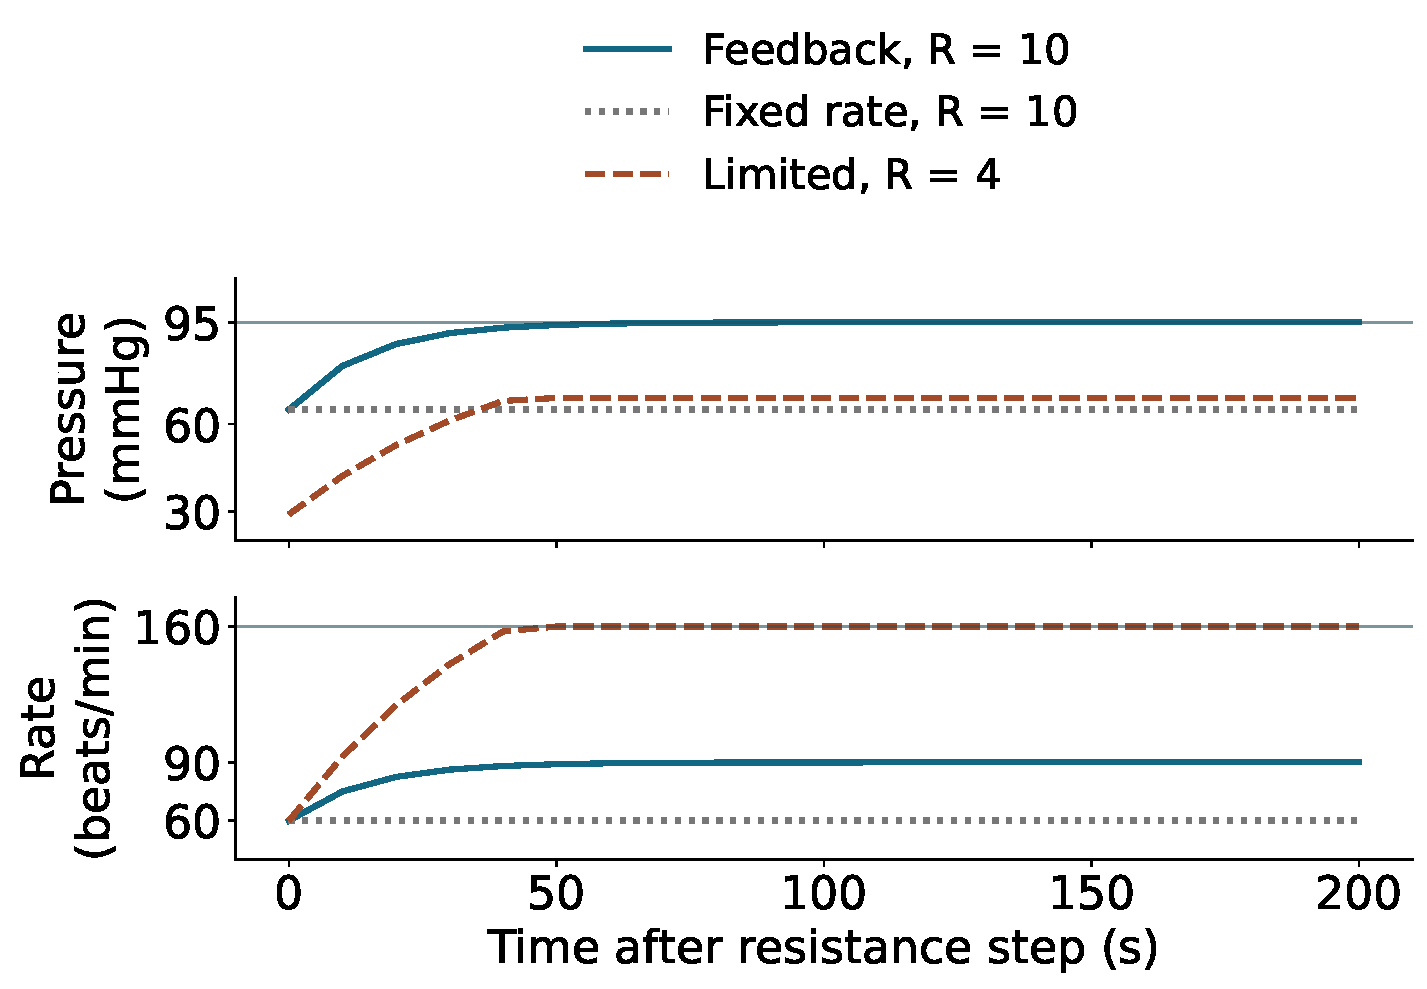
\includegraphics[width=.96\linewidth,height=.57\textheight,keepaspectratio]{feedback-response.pdf}\par\smallskip
{\small Synthetic step response at 10-second updates. Vs =\allowbreak{} 100 mL/beat, Pv =\allowbreak{} 5 mmHg, target 95 mmHg, gain 0.5 and rate bounds 40--160. Resistance drops from 15 to 10, or to 4 in the saturation comparison.}
\end{minipage}\end{center}
\section{An attainable target and a saturated controller}
\hypertarget{note-an-attainable-target-and-a-saturated-controller}{}\label{note:an-attainable-target-and-a-saturated-controller}
{\small \href{slides.html\#frame=the-rate-cannot-increase-without-bound\&step=1}{Slides for this section}}\par
The implemented rule limits rate to a permitted interval:
\begin{equation}H_{n+1}=\min\{H_{\max},\max\{H_{\min},H_n+k(P_*-P_n)\}\}.\end{equation}
With $H_{\min}=40$ and $H_{\max}=160\,\mathrm{beats/min}$, the target rate $90$ is attainable when $R=10$. But if $R=4$, then $a=0.4$ and the formal equilibrium requires
\[H_*=(95-5)/0.4=225\,\mathrm{beats/min}.
\]
The largest attainable pressure in the model is instead
\[P_{\max}=5+0.4(160)=69\,\mathrm{mmHg}.
\]
Once the rate reaches its upper bound, the remaining pressure error is $26\,\mathrm{mmHg}$. Increasing the gain cannot remove this limitation: it changes how the bound is reached, not the largest pressure the mechanism can produce. The simple geometric-error formula ceases to apply on a saturated step because the clipping operation changes the update.

Physiological pressure regulation involves more than this single control channel. Baroreceptor signaling can influence sympathetic and parasympathetic activity, vascular resistance, venous properties and cardiac behavior. The toy rule isolates the logic of negative feedback. It should not be read as a fitted baroreflex, a safe heart-rate prescription, or a claim that cardiac output always changes in one direction when resistance changes.
\section{A hydrostatic pressure difference}
\hypertarget{note-a-hydrostatic-pressure-difference}{}\label{note:a-hydrostatic-pressure-difference}
{\small \href{slides.html\#frame=the-weight-of-a-static-column\&step=1}{Slides for this section}}\par
Gravity introduces another pressure difference, even when fluid is stationary. Consider a vertical fluid column with cross-sectional area $A$, depth $d$, density $\rho$ and gravitational acceleration $g$. The fluid weight is $\rho Adg$. Force balance between its top and bottom gives
\begin{equation}(P_{\mathrm{bottom}}-P_{\mathrm{top}})A=\rho Adg,
\qquad P_{\mathrm{bottom}}-P_{\mathrm{top}}=\rho gd.\end{equation}
The area cancels. If $z$ increases upward, the equivalent signed relation is $P(z)-P(z_0)=-\rho g(z-z_0)$. With $\rho=1060\,\mathrm{kg/m^3}$ and $g=9.81\,\mathrm{m/s^2}$, a point half a meter below the reference is higher in hydrostatic pressure by $5199.3\,\mathrm{Pa}$, approximately $39.0\,\mathrm{mmHg}$ using $133.322\,\mathrm{Pa/mmHg}$.

A lower arterial point and a lower venous point can both have larger pressure. This does not give gravity a net pressure gain around a closed loop returning to its starting height: the height changes sum to zero. The hydrostatic column and the feedback recurrence are separate calculations in the companion. The height is not supplied as a controller input, and venous pooling or posture-dependent stroke volume is absent. Predicting a response to standing would require those missing connections, rather than simply adding $39$ to one displayed arterial pressure.
\bigskip
\section*{Exercises}
\par\noindent\begin{minipage}{\linewidth}
\subsection*{MC06-E1. One feedback step}
Use Vs =\allowbreak{} 80 mL/beat, H =\allowbreak{} 75 beats/min, Pv =\allowbreak{} 5 mmHg, R =\allowbreak{} 12 mmHg min/L, target 95 mmHg and gain 0.5. Bounds do not activate.

\textbf{a} Find output and current arterial pressure.

\end{minipage}\par\medskip
\textbf{b} Find error, next rate and next pressure.

\textbf{c} Identify two assumptions and a check on whether the correction moved toward the target.

\par\noindent\begin{minipage}{\linewidth}
\subsection*{MC06-E2. A target beyond the actuator}
Use Vs =\allowbreak{} 100 mL/beat, Pv =\allowbreak{} 5 mmHg, target 95 mmHg, resistance 5 mmHg min/L and allowed rate 40--160 beats/min.

\textbf{a} Calculate the rate required to attain the target.

\end{minipage}\par\medskip
\textbf{b} Find maximum achievable pressure and residual error.

\textbf{c} Explain why increasing the number of updates cannot remove this error, and name one omitted mechanism that might alter a biological response.

\par\noindent\begin{minipage}{\linewidth}
\subsection*{MC06-E3. Height and a project proposal}
Use rho =\allowbreak{} 1000 kg/m$^3$, g =\allowbreak{} 10 m/s$^2$ and 133.322 Pa/mmHg for an ideal static column.

\textbf{a} Find the pressure change 0.4 m below a reference point, in Pa and approximately mmHg.

\end{minipage}\par\medskip
\textbf{b} Explain why that pressure increment alone does not determine flow through a tissue bed.

\textbf{c} Write a bounded project question with an input, output, and verification check.

\section*{References}
\noindent\begin{minipage}{\linewidth}
Zan Ahmad, Fall 2023 HEART syllabus. Public PDF pp. 1--2, Course Topics and Course Expectations; editable syllabus pp. 2--3, project requirements.

\end{minipage}\par\medskip
\noindent\begin{minipage}{\linewidth}
Hoppensteadt and Peskin, Modeling and Simulation in Medicine and the Life Sciences, second edition. Printed pp. 21--24; PDF pp. 34--37, sections 1.7--1.8, sensitivity and baroreceptor-loop background.

\end{minipage}\par\medskip
\end{document}
